\documentclass{article}
\usepackage[final]{nips_2017}
\usepackage[utf8]{inputenc} % allow utf-8 input
\usepackage[T1]{fontenc}    % use 8-bit T1 fonts
\usepackage{hyperref}       % hyperlinks
\usepackage{url}            % simple URL typesetting
\usepackage{booktabs}       % professional-quality tables
\usepackage{amsfonts}       % blackboard math symbols
\usepackage{nicefrac}       % compact symbols for 1/2, etc.
\usepackage{microtype}      % microtypography
\usepackage{graphicx}
\usepackage{amsmath}
\usepackage{tikz}
\usetikzlibrary{positioning, shapes.geometric, arrows.meta}
\usepackage{natbib}
\bibliographystyle{unsrtnat}
\usepackage{hyperref}
\usepackage{float}

\title{Automated LaTeX Code Generation from Handwritten Mathematical Expressions \\
Category: Computer Vision}

\author{
  Jayaprakash Sundararaj \\
  \texttt{osjp@stanford.edu}  \\
  \AND
  Akhil Vyas \\
  \texttt{avyas21@stanford.edu}  \\
  \AND
  Benjamin Gonzalez-Maldonado \\
  \texttt{bengm@stanford.edu } \\
}

\begin{document}
% \nipsfinalcopy is no longer used

\begin{center}

\includegraphics[width=3cm, height=0.7cm]{CS230}
\end{center}

\maketitle

\begin{abstract}
Training a model that learns handwritten mathematical expressions from images and generates equivalent LaTeX code. The goal is experiment and study different model architectures (CNN, LSTM, etc) and hyper-parameters, evaluate the with different evaluation metrics, and share our finding.
\end{abstract}

\section{Introduction}	

Converting handwritten mathematical expressions into digital formats is time consuming, specifically LaTeX code. Our goal is to train a ML model that is capable of encoding handwritten notes and converting to the source code seamlessly. The input to our algorithm is an image of a handwritten mathematical expression. The challenge of our project is to convert an image to a text LaTeX sequence which will require the use of both computer vision and NLP techniques. We will use concepts related to these areas that we learn from this course to train the model. We will explore different evaluation metrics (text based, and image based), and share our findings.

% Explain the problem and why it is important. Discuss your motivation for pursuing this
% problem. Give some background if necessary. Clearly state what the input and output
% is. Be very explicit: “The input to our algorithm is an {image, amplitude, patient age,
% rainfall measurements, grayscale video, etc.}. We then use a {SVM, neural network, linear
% regression, etc.} to output a predicted {age, stock price, cancer type, music genre, etc.}.”
% This is very important since different teams have different inputs/outputs spanning different
% application domains. Being explicit about this makes it easier for readers. If you are using
% your project for multiple classes, add a paragraph explaining which components of the
% project were used for each class.

\section{Related work}
% [You should find existing papers, group them into categories based on their approaches,
% and discuss their strengths and weaknesses, as well as how they are similar to and differ
% from your work. In your opinion, which approaches were clever/good? What is the stateof-the-art?
% Do most people perform the task by hand? You should aim to have at least
% 5 references in the related work. Include previous attempts by others at your problem,
% previous technical methods, or previous learning algorithms. Google Scholar is very useful
% for this: https://scholar.google.com/ (you can click “cite” and it generates MLA, APA,
% BibTeX, etc.)]
\cite{schechter2017converting} investigated a variety of methods like neural networks, CNNs, Random Forests, SVMs, OCR, CGrp, and SA. However, most state of the art the methods utilize encoder-decoder architectures involving CNNs and LSTM architectures like \cite{genthial2016image}. In recent works like \cite{bian2022handwritten}, both left-to-right and right-to-left decoders are utilized. In our work, we will explore different hyper-parameters and model architectures such as attention mechanisms which were never tried before. 

\section{Dataset and Features}

We will use the datasets from two main repositories: \texttt{Im2latex-100k} (\cite{kanervisto_2016_56198}) and \texttt{Im2latex-230k} (\cite{gervais2024mathwritingdatasethandwrittenmathematical}). These datasets consist of images of mathematical formulas paired with their corresponding LaTeX code (two features). The Latex code is variable length.

The \texttt{Im2latex-100k} (\cite{kanervisto_2016_56198}) dataset, available at \href{https://zenodo.org/records/11230382}{Zenodo}, contains 100,000 image-formula pairs. Each image is in PNG format with a fixed size, and the formulas are extracted from ArXiv papers. This dataset is a cleaned-up version from the Cornell KDD competition (KDD Cup 2003). The \texttt{Im2latex-230k} (\cite{gervais2024mathwritingdatasethandwrittenmathematical}) 
 dataset, also known as \texttt{Im2latexv2}, contains 230,000 samples. It includes both OpenAI-generated and handwritten examples, further enhancing the diversity of the data. This dataset is available at \href{https://im2markup.yuntiandeng.com/data/}{Im2markup}. The training data format is \texttt{<image file name> <formula id>}.
 
 The dataset disk size is 849 MB. The images are gray scales with 50x200 pixels. The numbers of symbols (\autoref{fig:formula_length}) in the latex formulas vary from range varies from 1 to 150 symbols. Voabulary contains 540 symbols, refer \autoref{fig:vocab_freq_1} and \autoref{fig:vocab_freq_2} for the list of popular and least occurring symbols with their frequency.
 
\begin{figure}
    \centering
    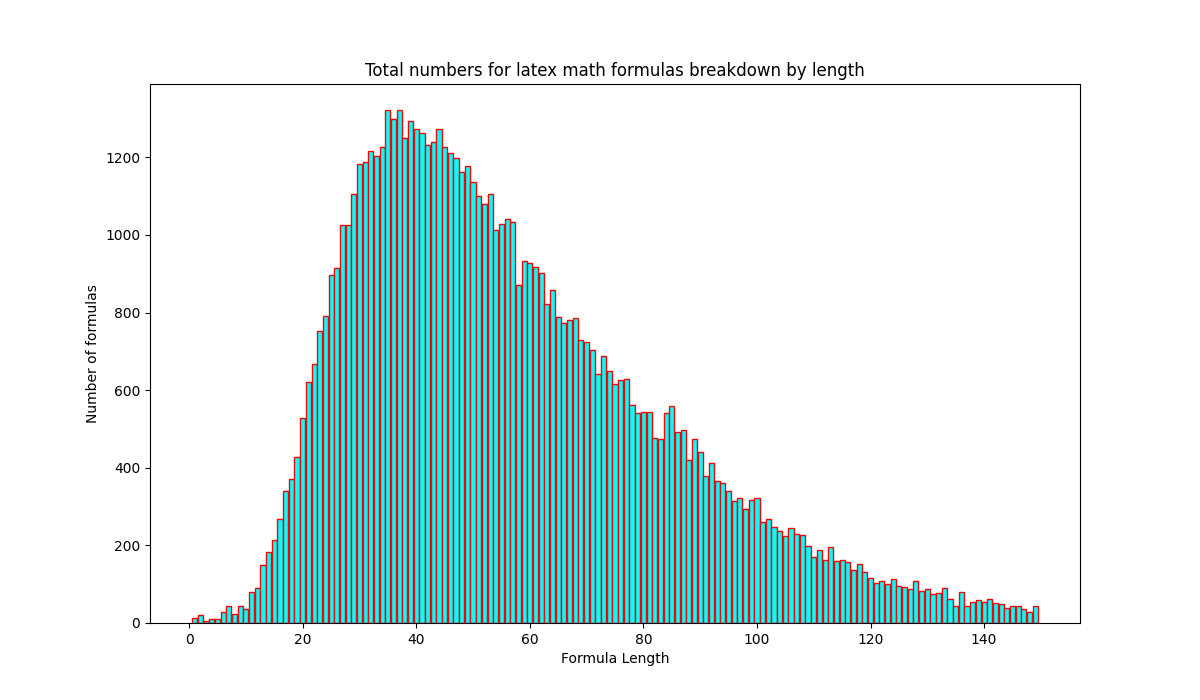
\includegraphics[scale=0.4]{fig_latex_formula_length.png}
    \caption{Formulas breakdown by length}
    \label{fig:formula_length}
\end{figure}


\section{Experiment}

In this project, we will use a Convolutional Neural Network (CNN) (\cite{OSheaN15}) combined with sequence-to-sequence (Seq2Seq) (\cite{6795963}) model to convert handwritten mathematical expressions into LaTeX code. The input to our algorithm is an image  \( I \), and the output is the corresponding LaTeX code, denoted as a sequence of tokens \( T = \{t_1, t_2, \dots, t_n\} \).

The Seq2Seq model, which consists of an encoder (the CNN) and a decoder (RNN, or LSTM), is trained for generate the LaTeX code token by token. At each time step \( t \), the decoder predicts the next token \( t_t \) given the previous tokens and the context vector \( c_t \). The probability distribution for the next token is computed as:
\[
P(t_t | t_{1:t-1}, c_t) = \text{softmax}(W_o h_t)
\]
where \( h_t \) is the hidden state of the decoder at time step \( t \), and \( W_o \) is a weight matrix.


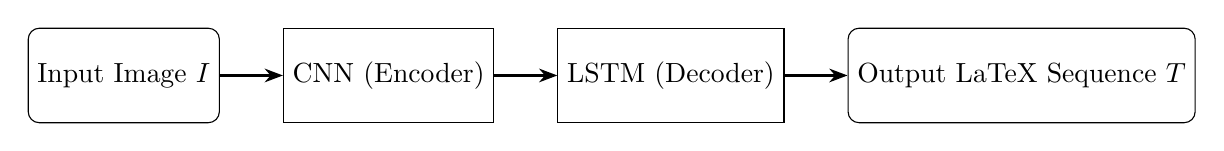
\begin{tikzpicture}[
    node distance=1cm, 
    every node/.style={rectangle, draw, minimum height=1.2cm, minimum width=1cm, align=center},
    arrow/.style={-Stealth, thick}
]

% Nodes
\node (input) [rounded corners] {Input Image \(I\)};
\node (cnn) [right=0.8cm of input] {CNN (Encoder)};
\node (lstm) [right=0.8cm of cnn] {LSTM (Decoder)};
\node (output) [right=0.8cm of lstm, rounded corners] {Output LaTeX Sequence \(T\)};

% Arrows
\draw [arrow] (input) -- (cnn);
\draw [arrow] (cnn) -- (lstm);
\draw [arrow] (lstm) -- (output);

\end{tikzpicture}

We'll use the cross-entropy loss function to optimize the model during training. Also, we plan to explore different attention mechanisms and extracting salient features as we iterate on the experimentation.

\subsection{Experiment Seup}
We use the single AWS P2 instance (tesla 80 GPU) for training. The training time varies between  

\subsection{CNN encoder and GRU/LSTM}
We use the LSTM instead of the GRU to compare the LSTM's performance improvement if any.

\subsection{LSTM with funetuning with pretrained Resnet50}
We use the LSTM instead of the GRU to compare the LSTM's performance improvement if any.

\subsection{Attention Model}
  [WIP] We're in the middle of using attention mechanism to experiment with attention mechanism for the model to learn complex dependencies.
  
\subsection{Beam Search Instead of Greedy Decoding}
  [WIP] We're in the middle of using attention mechanism to experiment with attention mechanism for the model to learn complex dependencies. 

\section{Experiments and Evaluation}

We will use the following metrics to evaluate the performance of the model for the LaTeX code generation task. The text based metrics compare the original LaTeX code with generated LaTeX code, however, the image based metrics compare the PDF images generated from original and generated LaTeX code.

\begin{itemize}
    \item Text Metrics: \textbf{BLEU Score} (\cite{papineni-etal-2002-bleu})
    \item Text Metrics: \textbf{Levenshtein Distance}
    \item Image metrics: Compute the \textbf{accuracy} between images generated from original latex code and generated latex code. 
\end{itemize}

The experimentation will involve choosing different CNN layers (striding, pooling), learning rate, mini batch size. 

\section{Remaining work for Final Project}

\textbf{Re-weighted mis-predicted training example}: We're aiming to inspect the accuracy losses and ensure that mis-predicted examples are correctly identified with increased weighting. 

\textbf{Image based evaluation metrics}: We have accuracy based metrics implemented, and edit distance based and BLEU Score based metrics implemented. We're planning to implement \textbf{Image Based} evaluation metrics as two different latex formulas can mean the same formula.

\section{Contributions}

\textbf{Jayaprakash Sundararaj}: Initial report, researching the dataset and existing methods. Implementing the full CNN and LSTM as a baseline. Extending to pre-trained ResNet50 model with finetuning.

\textbf{Akhil}: Ideation, Setting AWS/GPU setup, Extending to full CNN and GRU as a baseline, Extending to attention/transformer architecture (work in progress).

\textbf{Ben}: TODO


\medskip

\nocite{*}
\bibliography{sample}
\small


\section{Appendix}

\begin{figure}[H]
    \centering
    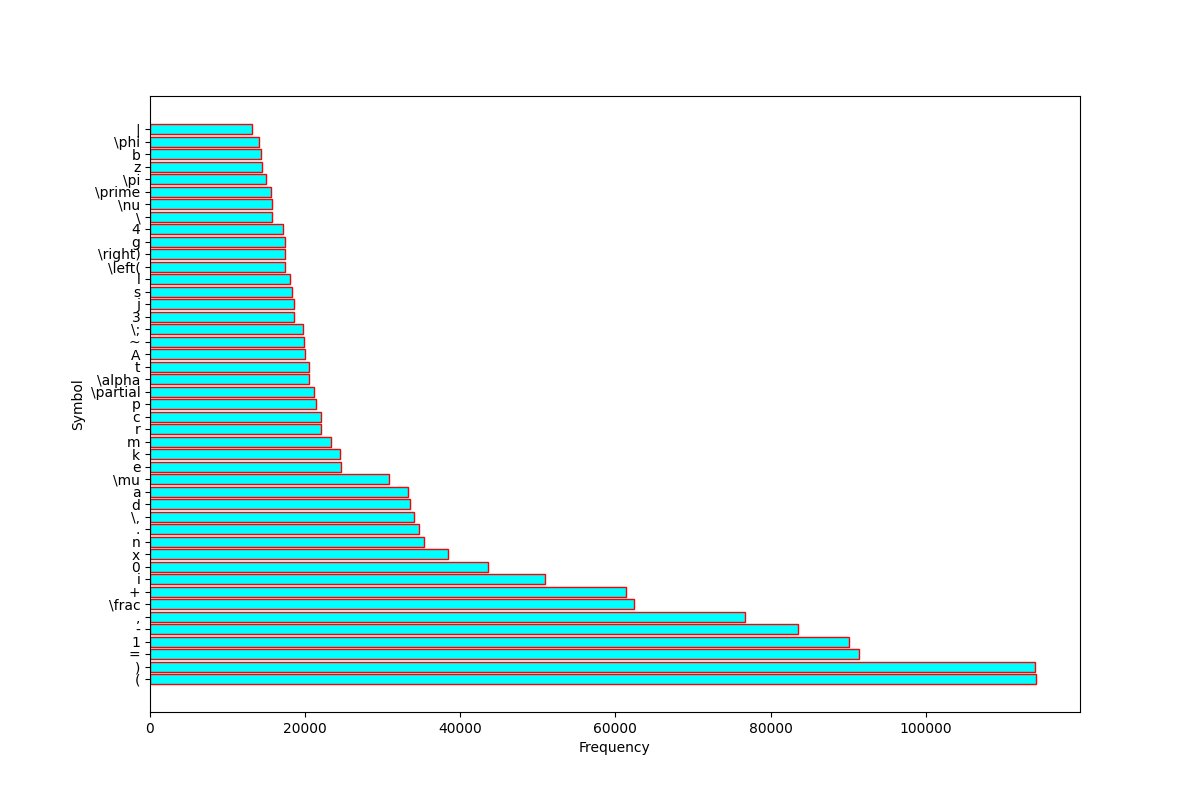
\includegraphics[scale=0.4]{fig_vocabs_frequency_1.png}
    \caption{Dataset: Most popular symbols and frequencies.}
    \label{fig:vocab_freq_1}
\end{figure}

\begin{figure}[H]
    \centering
    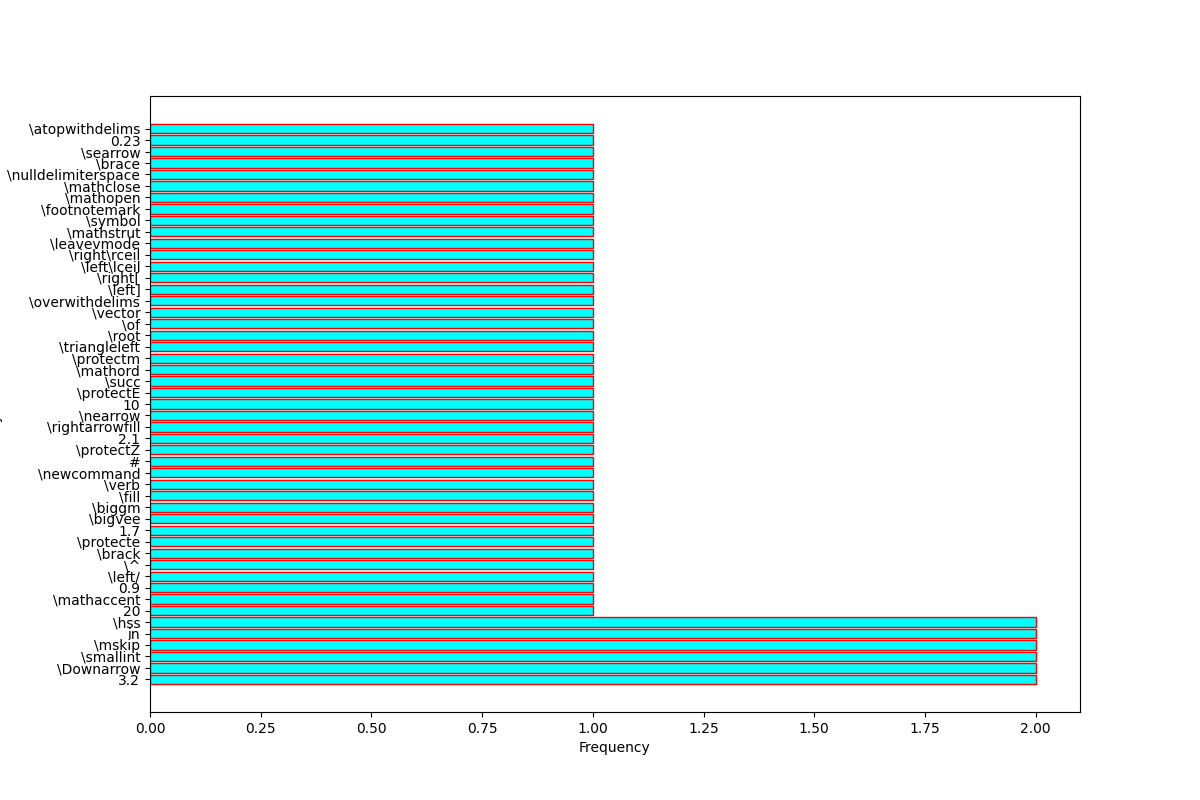
\includegraphics[scale=0.4]{fig_vocabs_frequency_2.png}
    \caption{Dataset: Least popular symbols and frequencies.}
    \label{fig:vocab_freq_2}
\end{figure}

\end{document}